% !TEX root=../report.tex

\section{Interaction with end users using editors}

In the introduction we claimed to create a language to model \emph{interactive} workflows.
By interaction we mean \emph{communication with people using the developed system}.
These \emph{end users} should be able to enter information into the system,
change it, clear it, reenter it, etc.
To do this, we introduce the concept of an \emph{editor}.

Editors may or may not contain a current value.
When an editor has a value, it can be \emph{changed} or it can be \emph{emptied}.
When it is empty, a value can be \emph{filled}.
This is depicted as a state diagram in \autoref{fig:editor-state} below.

\begin{figure}
  \centering
  \includegraphics[width=0.5\textwidth]{figures/drawings-crop.pdf}
  \caption{Possible states of an editor and its transitions.}
  \label{fig:editor-state}
\end{figure}

One can consider editors as an abstraction over widgets in a \GUI,
form fields on a webpage,
or even sensors plugged into the system.
Take for example an entry for text.
Users can enter a string, change it, remove it, enter another string, and so on.
With editors we try to capture this \emph{constantly changing} nature of user input.
Also, because editors are \emph{typed},
they are only allowed to contain information of the right format.

How exactly information is entered is not of great importance.
This could be an input field for a string,
a switch for a boolean,
a spin box for an angle,
or even a map with a pin for a location.
\Autoref{fig:editor-examples} depicts these examples.
In it's most banal form,
an editor is a line of text entered at a terminal and parsed to match a string, boolean, angle or location value.

\begin{marginfigure}
  \centering
  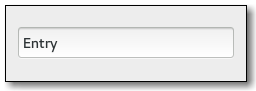
\includegraphics[width=0.7\marginwidth]{figures/text-entry}
  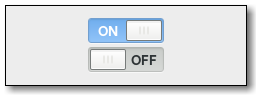
\includegraphics[width=0.7\marginwidth]{figures/switch-button}
  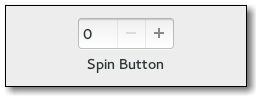
\includegraphics[width=0.7\marginwidth]{figures/spin-button}
  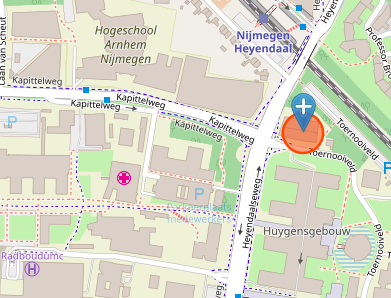
\includegraphics[width=0.7\marginwidth]{figures/map}
  \caption{
    Some examples of editors.
    From top to bottom:
    a text field for strings,
    a switch for booleans,
    a spin box for angles,
    and a map for locations.
  }
  \label{fig:editor-examples}
\end{marginfigure}

\begin{margintext}{Aside: About stability}
  A short side note to the iTasks guru.
  Maybe you think: \enquote{I know these different states! This is stability!}
  Yes and no.
  I already mentioned in the introduction we won't use the notion of stability in our system.
  Although the state diagram in \autoref{fig:editor-state} looks like the state diagram for stability,
  it has absolutely nothing to do with it.

  First, stability has \emph{three} states:
  \begin{enumerate*}
    \item stable,
    \item unstable, and
    \item no value.
  \end{enumerate*}
  These are depicted below.
  Editors have only \emph{two}:
  \begin{enumerate*}
    \item valued, and
    \item unvalued.
  \end{enumerate*}

  \includegraphics[width=\marginwidth,page=2]{figures/drawings-crop.pdf}

  Second,
  it is possible for an editor to go from a valued to an unvalued state and back again,
  but there is no way to mark an editor as stable.
  It is a bit like using only the unstable part of above state diagram.
  This is about the only resemblance.

  Third,
  the state diagram in \autoref{fig:editor-state} is about \emph{editors only}.
  A value in our system is \emph{always there}.
  Because values are just values,
  as we are custom from lambda calculus and other functional programming languages,
  stability does not propagate through our whole language.
  Editors are the \emph{only} entities in our language that are allowed to contain a value or not.
  This doesn't change anything to values in our underlaying expression language.

  I can't stress it enough, so here it is again:
  \begin{quote}
  Editors live on the \emph{task level} of our language,
  values live on the \emph{expression level}.
  We do not change \emph{anything at all} on the expression level when introducing tasks.
  \end{quote}
\end{margintext}


\subsection{Syntax and typing}

At the core,
an editor is a container holding a value
or holding nothing.
For this purpose, we extend our task language with two constructs:
a valued editor $\Edit e$ and an unvalued editor $\Enter \beta$.
\begin{grammar}
  Pretasks
    & p & ::=& \ldots       & \\
    &   &\mid& \Edit e      & – valued editor \\
    &   &\mid& \Enter \beta & – unvalued editor \\
\end{grammar}

Valued editors contain an expression $e$.
Therefore they inherit the type of $e$,
but embedded in the container type $\Task$.
For now, we only accept expressions of a basic type $\beta$ as a value of an editor.
This is expressed by the following typing rule for valued editors.
\begin{equation*}
  \userule{T-Edit}
\end{equation*}

Unvalued editors do not have a value,
and therefore do not wrap an expression.
Because we strive to a fully typed system,
we have two options to type unvalued editors:
\begin{enumerate*}
  \item let the unvalued editor have a polymorphic type;
  \item annotate unvalued editors with a type and use that. \label{itm:annotate}
\end{enumerate*}

The first option sounds appealing.
However, consider the following use case.
We start with an editor containing the value two: $\Edit 2$.
The user can change this value, as long as it is an integer,
for example to five: $\Edit 5$.
Clearing the value results in an unvalued editor: $\Enter$.
Now, are we allowed to enter a value of some other type?
That is, can we now enter a string?
This would change the type of the editor!

Therefore,
we need to keep track of the type of values that can be entered into an unvalued editor
and we choose option (\ref{itm:annotate}).
The typing rule becomes:
\begin{equation*}
  \userule{T-Enter}
\end{equation*}

Some examples of editors expressible in our language:
\begin{itemize}
  \item $\Edit 2$ is a valued editor which contains the integer value $2$.
  \item $\Enter \String$ is an unvalued editor,
    waiting for users to enter some string.
  \item $\Edit ((\lambda x . x)\ 5)$ is a valued editor which,
    after evaluation, will contain the value $5$.
    (We will discuss evaluation of editors in the next section.)
\end{itemize}


\subsection{Evaluating pretasks to tasks}
\label{sec:tasks-vs-pretasks}

Till now, syntactically we only talking about \emph{pretasks}.
Now the time has come to talk about \emph{real} tasks!
Well, about \emph{syntactically real} tasks.
\begin{grammar}
  Tasks
    & t & ::=& \ldots       & \\
    &   &\mid& \Edit v      & – valued editor \\
    &   &\mid& \Enter \beta & – unvalued editor \\
\end{grammar}

So what is the difference with pretasks?
The subtle change from $\Edit e$ to $\Edit v$ in the valued editor.
That is, an editor with an arbitrary (although well typed) expression $e$,
versus an editor with an (evaluated) value $v$.
Coming from one to the other is done by the evaluation relation we introduced in \autoref{sec:evaluation}.

There are two rules we need to add for this semantic arrow to accomplish this:
one for valued and one for unvalued editors.
\begin{equation*}
  \userule{E-Edit} \qquad \userule{E-Enter}
\end{equation*}
Rule \refrule{E-Edit} uses the big step semantics from our base language ($\evaluate$)
to evaluate the wrapped expression $e$ to a value $v$ and rewraps it in an editor.
Rule \refrule{E-Enter} has nothing to evaluate and just keeps the unvalued editor as is.

Summarising, pretask $p$ allow us to syntactically write down arbitrary expressions inside a valued editor,
or any other pretask we will define in the future.
Tasks $t$ are pretasks \emph{after evaluation} using the relation $\evaluate$.
With other words:
\begin{itemize}
  \item
    Pretasks $p$ are task expressions.
  \item
    Tasks $t$ are a syntactical subset of pretasks $p$.
    They are values with respect to evaluation, i.e. the relation $\evaluate$.
\end{itemize}


\subsection{Handling inputs}
\label{sec:handling}

To change values in an editor,
we should interact with the user by some kind of interface.
In a graphical setting,
we can present the user an input box.
The user can then change and clear values continuously.
In a text oriented world,
we can print out the current value of an editor
and prompt the user for a new value
or a command to empty the editor.

To abstract away from the user interface,
we introduce an event system.
It does not matter how these events are sent to the application.
This can be by pushing a button,
entering text in an input box,
committing some text on a command line,
sending it over a web socket,
etc.

\begin{margintext}{Aside: Accessing events}
In a previous attempt to build a semantics for \TOP,
\textcite{theses/radboud/VinterHviid18} also used the notion of events.
However, \citeauthor{theses/radboud/VinterHviid18} made events part of the task layer.
This means the programmer has access to events using a \texttt{getEvent} function call.

In this work,
we deviate from above idea.
We use labeled transitions in the same way as \textcite{school/maktoberdorf/PeytonJones01},
who gives denotational semantics to the Haskell \IO monad.
Therefore events live on the \emph{semantic level} only
and they are \emph{not} accessible from within our language.
\end{margintext}

We define a new syntactic category of \emph{events} $h$.
For now, they only contain \emph{actions} $a$.
We will introduce more events and actions in later sections.
\begin{grammar}
  Inputs
    & i & ::=& a      & – action \\
  Actions
    & a & ::=& v      & – change editor to value \\
    &   &\mid& \Empty & – empty an editor \\
\end{grammar}

As we already discussed before,
there are three actions that can be handled by editors:
\begin{enumerate*}
  \item filling in an unvalued editor;
  \item changing the value; or
  \item clearing the value.
\end{enumerate*}
We choose to merge the first two, filling and changing, into one action.
The value of an editor, empty or not, can be changed to a value $v$ by just sending the value as an action.
To empty a valued editor, we send the $\Empty$(mpty) action.

Handling inputs is done by a new semantic relation.
This small step relation takes a task $t$ and an event $h$ which results in a new task $t'$.
We write
\begin{equation*}
  \boxed{\RelationH}
\end{equation*}
Formalising the states and transitions shown in \autoref{fig:editor-state},
we need three rules to describe editors.
\begin{equation*}
  \userule{H-Change} \qquad \userule{H-Empty} \qquad \userule{H-Fill}
\end{equation*}
Note that the conditions to the right of the rules take care of typing.
Only when the entered value $v'$ has the same type $\beta$ as the original value $v$ we can change a valued editor.
In case of an unvalued editor,
the entered value $v'$ needs to have the same type as the type annotation $\beta$.
These conditions make sure the type of the entered value and the type of the editor are always the same.


\subsection{Example: an interactive session}

Now that we have introduced our first kind of task,
we can make a dull but interactive example of a workflow.
How could an interactive session with the user look like when we start with a simple workflow of one editor,
containing the value two?
\begin{align*}
    & \Edit 2 \\
  \handle{5} & \hint{change value to five} \\
    & \Edit 5 \\
  \handle{\Empty} & \hint{clear the current value} \\
    & \Enter \Int \\
  \handle{50} & \hint{enter the value fifty} \\
    & \Edit 50 \\
  \handle{\str{Bye}} & \hint{sending a string won't work, the types don't match} \\
    & \Edit 50 \\
  \handle{10} & \hint{change value to ten} \\
    & \Edit 10
\end{align*}

Next we will introduce sequential composition of tasks to spice up our workflows a bit,
but not before we have introduced the other basic task in our toolbox.
